\documentclass[12pt,a4paper]{article}
\usepackage{fullpage}
\usepackage[margin=2cm]{geometry}
\usepackage{amsmath}
\usepackage{subfig}
\usepackage{graphicx}
\usepackage[justification=centering]{caption}
\begin{document}
\title{A convolutional neural network on Beetles dataset }
\author{LE Van Linh and BEURTON-AIMAR Marie}
\date{October, 2017}
\maketitle
\begin{abstract}
In this study, we present a convolutional neural network (CNN) which is used to predict the landmarks on beetle's images.  The model is designed as a pipeline of the layers. It is evaluated on five datasets of beetle: \textit{left mandible, right mandible, pronotum, body, and head}. The models which used to predict the landmarks for each beetle's part have the same structures but the output at the last layer is modified to suitable with the number of landmarks that it should be predicted. For each dataset, a number of $260$ images are used to train and validate, the remaining images are used to test the output model. The evaluation is the correlation coefficient between the manual coordinates (which given by the biologist) and the predict coordinates. Besides, a statistic based on the distances between the manual landmarks and predicted landmarks are also calculated. The model is implemented by Python on Lassagne framework\cite{lasagne}.
\end{abstract}

\section{Convolutional neural network}
\subsection{Architecture}
The network includes three convolutional(CONV) layers followed by three maximum pooling(POOL) layers, four dropouts(DROP) layers, and three full connected(FC) layers (Fig.\ref{pmodel}). The input of the network is the gray-scale image with the size of $256 \times 192$. The depth of network can be expressed by increasing of the deep at each convolutional layer. They are increased from $32, 64,$ and $128$ from the first CONV layer to the third CONV layer with different filter sizes. While, the filter sizes are kept in the same size for every POOL layers. The dropout ratios of the DROP layers increase from the first to the end: $0.1, 0.2, 0.3, $ and $0.5$. At the end of the network, three full connected are set up to predict the landmarks. The first two FC layers have the same outputs($1000$) while the output at the last FC has been change to correspond with the number of landmarks. The detail parameters at each layer are presented in Appendix \ref{apa}. The model is implemented by Lassagne framework\cite{lasagne}.
\begin{figure}[h!]
	\centering
	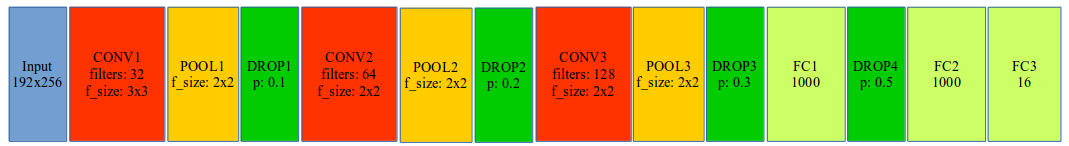
\includegraphics[scale=0.45]{images/model3_dropout}
	\caption{The illustration of the convolutional neural network}
	\label{pmodel}
\end{figure}
\subsection{Parameters}
The model is trained with $5000$ \texttt{epochs} and \texttt{batch size} of $128$. For each epoch, the dataset is randomly split into training set and validation set with the ratio of $0.6:0.4$. The \texttt{learning rate} and \texttt{momentum} are initialized to $0.03$ and $0.9$, respectively. During training, they are re-calculated to adjust with the remaining epochs. All the initial parameters are shown in the Table \ref{initparameters}.
\begin{table}[h!]
	\centering
	\begin{tabular}{l l l}
	Parameter & Initial value & End value \\ \hline
	Epochs & 5000 &  \\ \hline
	Training batch size & 128 & \\ \hline
	Testing batch size & 128 & \\ \hline
	Learning rate & 0.03 & 0.0001 \\ \hline
	Momentum & 0.9 & 0.9999 \\ \hline
	Training data & 0.6 & \\ \hline
	Validation data & 0.4 &  \\ \hline
	\end{tabular}
	\caption{The network parameters in proposed model}
	\label{initparameters}
\end{table}
\section{Data}
The beetle dataset includes the images of five parts: \textit{left mandible, right mandible, pronotum, body, and head}. For each part, a collection of \textbf{293} images are collected. However, the number of the images in each part are changed after checking to suppress the not-working images (i.e empty image, broken object). Table \ref{datatable} shows the number of available images in each part and the number of the images in each process.
\begin{table}[h!]
	\centering
	\begin{tabular}{l c c c}
	Part & Total available images & Training + Validation & Testing \\ \hline
	Left mandible & 286 & 260 & 26 \\ \hline
	Right mandible & 290 & 260 & 30 \\ \hline
	Body & 293 & 260 & 33 \\ \hline
	Head & 293 & 260 & 33 \\ \hline
	Pronotum & 293 & 260 & 33 \\ \hline
	\end{tabular}
	\caption{The number of available images and the number of the images which used to train (and validate) and test}
	\label{datatable}
\end{table}~\\
Because the number of the images are limited (just $260$ color images), it does not enough to use for training process. Additional, the models are worked on gray-scale images. So, we applied some rules to enlarge the dataset for each part. The first rule is adding a constant value to a channel of RGB image, we will have a new RGB image. For example, from an original $RGB$ image, if we add $10$ to red channel, we will have a new image $(R+10)GB$. Then, we apply the same rule with blue and green channel, we will obtain two new images: $R(G+10)B$ and $RG(B+10)$. By that way, from an RGB image, we can generate three RGB images by adding a constant to each channel(each time just change to a channel). The second rule is splitting the channels of RGB image (because the models work on gray-scale). It means that we can generate six versions from an original image. At the end, the number of the image in the training data is $ 260 \times 7 = 1820$ images (six versions and original). Before giving to the models, the images are down-sampled with the size of $256 \times 192$. The number of the images in training set and validation set are splitted automatically by the model's parameter.
\section{Experiments}
In practical, convergence is usually faster if the average of each input variable over the training set is close to zero. Because the values of the pixels and the coordinates of the landmarks are positive. If we consider that we stay at the a layer of the network, and the weights are updated by an amount proportional to $\delta x$($\delta$ is the scalar error at the layer and $x$ is the input vector). When the input vectors are positive, the updates of weights that feed into the layer will be the same sign($sign(\delta)$), it means that the weights can only all decrease or all increase together for a given input. That, if the weight vector change direction, it can only do by zigzagging which is inefficient and thus slow down learning. Therefore, it is good to shift the inputs so that the average over the training set is close to zero. Moreover, when the input is set closed with zero, it will more suitable with the sigmoid activation function\cite{lecun2012efficient}. So, \textit{the brightness of the image is normalized to $[0,1]$, instead of $[0,255]$. And, the coordinates of the landmarks are normalized to $[-1,1]$, instead of $[0,256]$ and $[0,192]$ before giving to the network}.

For each part, the network is training and validation with many times (called round). In each round, the training dataset is changed following the way to choose the test dataset (i.e circular). At the end, we can obtain the predicted landmarks of all images in this part by combining all the  testing images corresponding with the training model. 

The predicted landmarks are evaluated by two ways: calculating correlation coefficient and computing the statistic based on the number of landmarks has well prediction.
The correlation coefficient is calculated by using three methods: Pearson\cite{pallant2013spss}, Spearman\cite{myers2010research}, and Kendall\cite{kendall1938new}. The well prediction statistic is computed based on the distance between manual and predicted landmark. Firstly, the distance between manual and prediction one is calculated. Then, the average distance of this landmark on all images has been computed. A predicted landmark is considered as well prediction if the distance between it and the corresponding manual is less than average value. The average distance of each landmark of each beetle's part is shown in Appendix \ref{apavgdistance}. Besides, the well prediction statistics of mandibles have been compared with the previous result\cite{le:hal-01571440}.

This section presents the experimental on all parts of Beetle. For each part, we present the losses (training and validation), the correlation coefficient and the statistic of well prediction. All of the experiment results have been provided on GitHub\footnote{https://github.com/linhlevandlu/cnnBeetles/tree/master/data}(Appendix \ref{apb}).
\pagebreak
%left mandible, right mandible, pronotum, body, and head
\subsection{Left mandible part}
Table \ref{mgloss} shows the information during training and validation on left mandible.
\begin{table}[h!]
	\centering
	\begin{tabular}{l p{2cm} p{2.4cm} p{2.6cm} p{2.2cm} p{2.2cm}}
	Round & Total images & Testing index (from-to) & Training index (from-to) & Training loss & Validation loss \\ \hline
	r1 & 286 & 1-26 & 27-286 & 0.00073 & 0.00148 \\ \hline
	r2 & 286 & 27-52 & remaining & 0.00074 & 0.00149 \\ \hline
	r3 & 286 & 53-78 & remaining & 0.00074 & 0.00177 \\ \hline
	r4 & 286 & 79-104 & remaining & 0.00068 & 0.00141 \\ \hline
	r5 & 286 & 105-130 & remaining & 0.00077 & 0.00231 \\ \hline
	r6 & 286 & 131-156 & remaining & 0.00070 & 0.00180 \\ \hline
	r7 & 286 & 157-182 & remaining & 0.00063 & 0.00125 \\ \hline
	r8 & 286 & 183-208 & remaining & 0.00062 & 0.00104 \\ \hline
	r9 & 286 & 209-234 & remaining & 0.00067 & 0.00173 \\ \hline	
	r10 & 286 & 235-260 & remaining & 0.00067 & 0.00145 \\ \hline
	r11 & 286 & 261-286 & remaining & 0.00072 & 0.00188 \\ \hline
	\end{tabular}
	\caption{The training loss and validation loss at each training round of left mandible}
	\label{mgloss}
\end{table}~\\
Which:
\begin{itemize}
	\item \textbf{Round}: indexing training round
	\item \textbf{Total images}: total images of left mandible
	\item \textbf{Testing index}: indexing of the images that chosen to test set.
	\item \textbf{Training index}: indexing of the images that chosen to train and valid set.
	\item \textbf{Training loss}: training loss at a round
	\item \textbf{Validation loss}: validation loss at a round
\end{itemize}~\\
Fig.\ref{lossmgcurves} shows the curves of training and validation losses of two rounds of left mandible.
\begin{figure}[h!]
\centering
\subfloat[Round 1]{\label{model1loss2}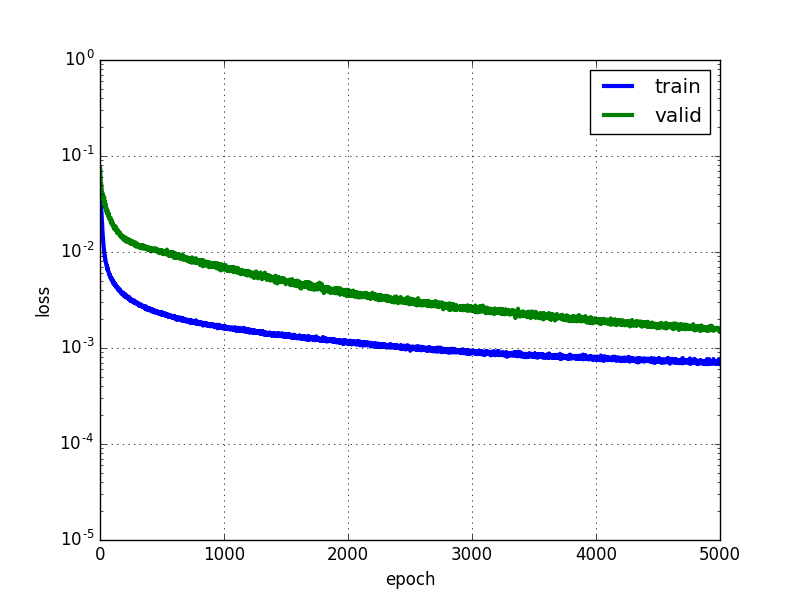
\includegraphics[width=0.5\textwidth]{./images/cnnmodel3_5000_mg_1000_output_v10}}~~
\subfloat[Round 8]{\label{model2loss2}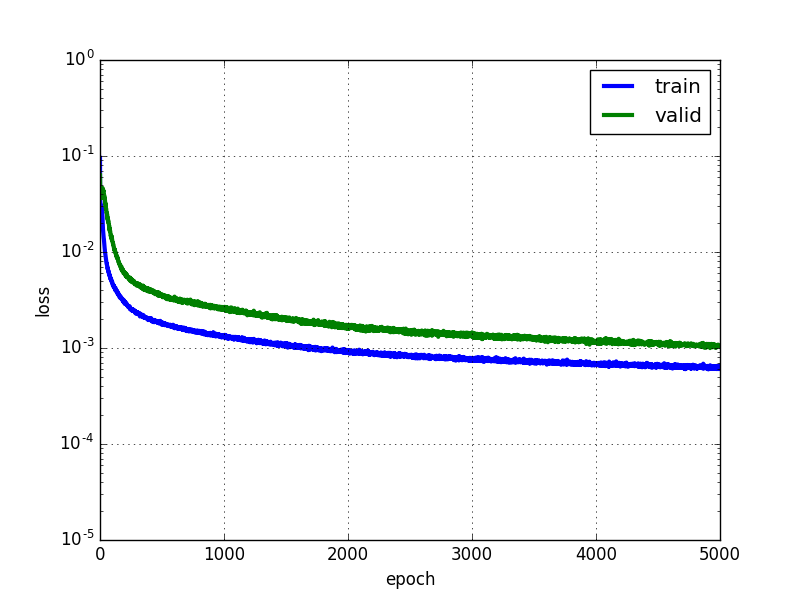
\includegraphics[width=0.5\textwidth]{./images/cnnmodel3_5000_mg_1000_output_v18_loss}}
\caption{The losses curves of training and validation of two training rounds of left mandible  }
\label{lossmgcurves}
\end{figure}~\\[2cm]
The correlation coefficient results on left mandibles are shown in Table \ref{corrmg}.
\begin{table}[h!]
	\centering
	\begin{tabular}{l c c}
		Method & x correlation & y correlation \\ \hline
		Pearson & $0.9781574$ & $0.9875064$ \\ \hline
		Spearman & $0.983688$ & $0.9800946$ \\ \hline
		Kendall & $0.9136765$ & $0.8932026$ \\ \hline
	\end{tabular}
	\caption{The correlation between manual and predicted landmarks on left mandible images}
	\label{corrmg}
\end{table}~\\
Fig.\ref{mgfig} shows the proportions of well predicted landmarks on left mandibles.
\begin{figure}[h!]
	\centering
	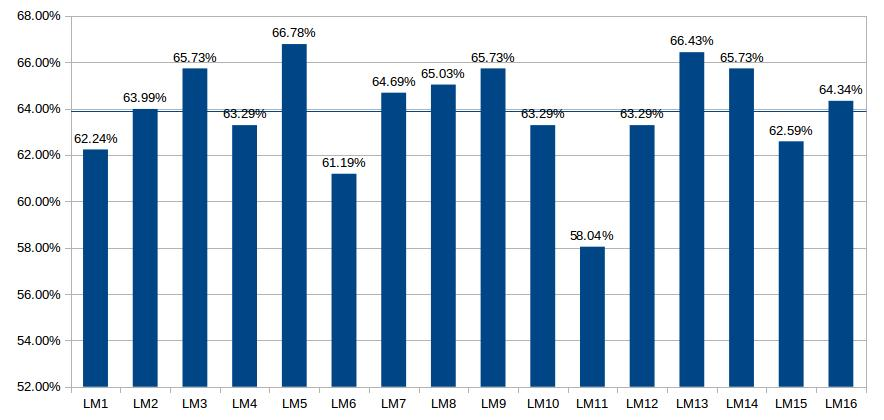
\includegraphics[scale=0.55]{images/mg}
	\caption{The proportion of well predicted landmarks on left mandibles}
	\label{mgfig}
\end{figure}~\\
Fig.\ref{mgfig2} shows the proportions of well prediction on MAELab \cite{le:hal-01571440}.
\begin{figure}[h!]
	\centering
	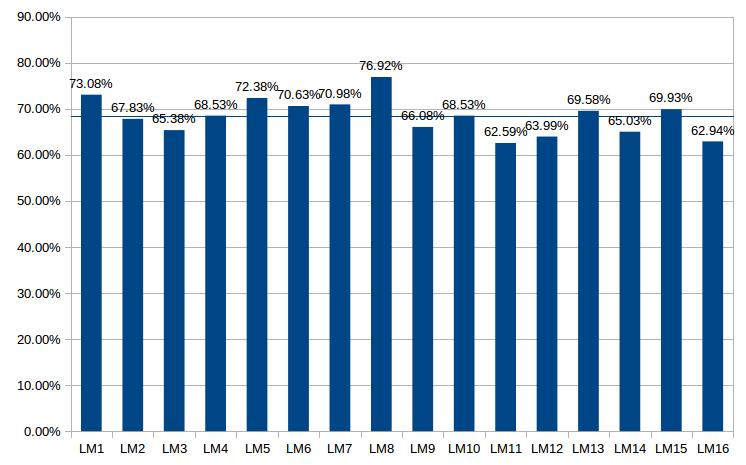
\includegraphics[scale=0.53]{images/mgSIFT}
	\caption{The proportion of well predicted landmarks on left mandibles(MAELab)}
	\label{mgfig2}
\end{figure}~\\
\subsection{Right mandible part}
The information of each training round on right mandible is shown in Table \ref{mdloss}.
\begin{table}[h!]
	\centering
	\begin{tabular}{l p{2cm} p{2.4cm} p{2.6cm} p{2.2cm} p{2.2cm}}
	Round & Total images & Testing index (from-to) & Training index (from-to) & Training loss & Validation loss \\ \hline
	r1 & 290 & 1-30 & 31-290 & 0.00075 & 0.00162 \\ \hline
	r2 & 290 & 31-60 & remaining & 0.00081 & 0.00208 \\ \hline
	r3 & 290 & 61-90 & remaining & 0.00076 & 0.00158 \\ \hline
	r4 & 290 & 91-120 & remaining & 0.00075 & 0.00167 \\ \hline
	r5 & 290 & 121-150 & remaining & 0.00079 & 0.00206 \\ \hline
	r6 & 290 & 151-180 & remaining & 0.00080 & 0.00263 \\ \hline
	r7 & 290 & 181-210 & remaining & 0.00081 & 0.00245 \\ \hline
	r8 & 290 & 211-240 & remaining & 0.00080 & 0.00194 \\ \hline
	r9 & 290 & 241-270 & remaining & 0.00079 & 0.00157 \\ \hline	
	r10 & 290 & 271-290 & remaining & 0.00082 & 0.00242 \\ \hline
	\end{tabular}
	\caption{The training loss and validation loss at each training round of right mandible}
	\label{mdloss}
\end{table}~\\
Fig.\ref{lossmdcurves} shows the curves of training and validation losses of two rounds on right mandible.
\begin{figure}[h!]
\centering
\subfloat[Round 1]{\label{model1loss2}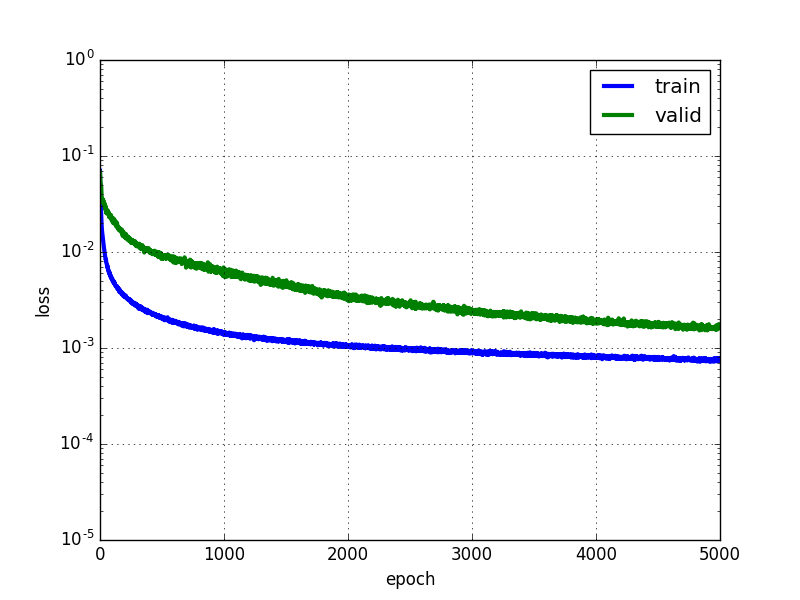
\includegraphics[width=0.5\textwidth]{./images/cnnmodel3_5000_md_1000_output_v10_loss}}~~
\subfloat[Round 8]{\label{model2loss2}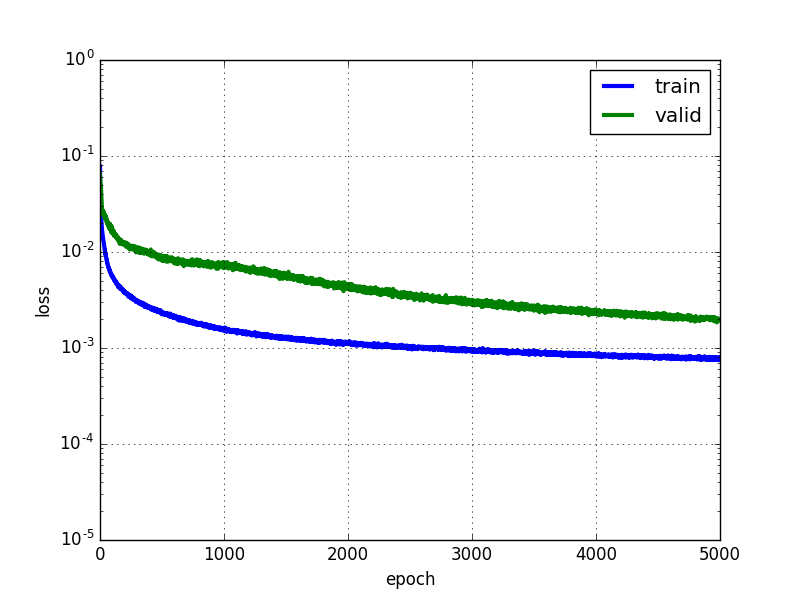
\includegraphics[width=0.5\textwidth]{./images/cnnmodel3_5000_md_1000_output_v18_loss}}
\caption{The losses of two training rounds of right mandible  }
\label{lossmdcurves}
\end{figure}~\\
Table \ref{corrmd} shows the correlation coefficient between manual landmarks and predicted landmarks on right mandibles.\\[0.1cm]
\begin{table}[h!]
	\centering
	\begin{tabular}{l c c}
		Method & x correlation & y correlation \\ \hline
		Pearson & $0.9852194$ & $0.9858498$ \\ \hline
		Spearman & $0.9863889$ & $0.983251$ \\ \hline
		Kendall & $0.9104557$ & $0.898321$ \\ \hline
	\end{tabular}
	\caption{The correlation between manual and predicted landmarks on right mandible images}
	\label{corrmd}
\end{table}~\\
Fig.\ref{mdfig} shows the proportions of well predicted landmarks on right mandibles.
\begin{figure}[h!]
	\centering
	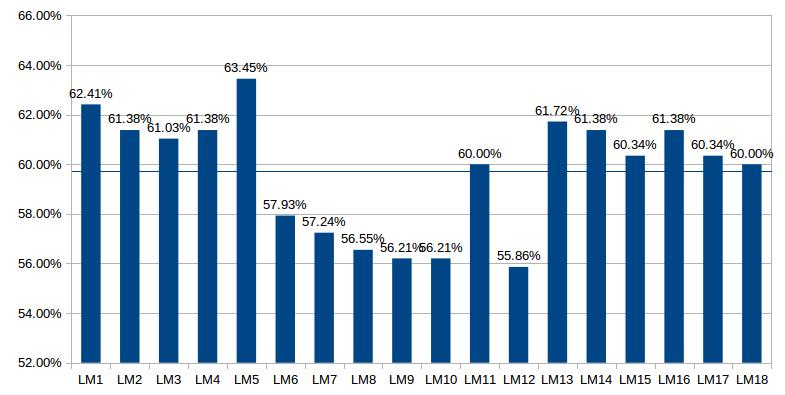
\includegraphics[scale=0.65]{images/md}
	\caption{The proportion of well predicted landmarks on right mandibles}
	\label{mdfig}
\end{figure}~\\[2cm]
Fig.\ref{mdfig2} shows the proportions of well prediction on MAELab \cite{le:hal-01571440}.
\begin{figure}[h!]
	\centering
	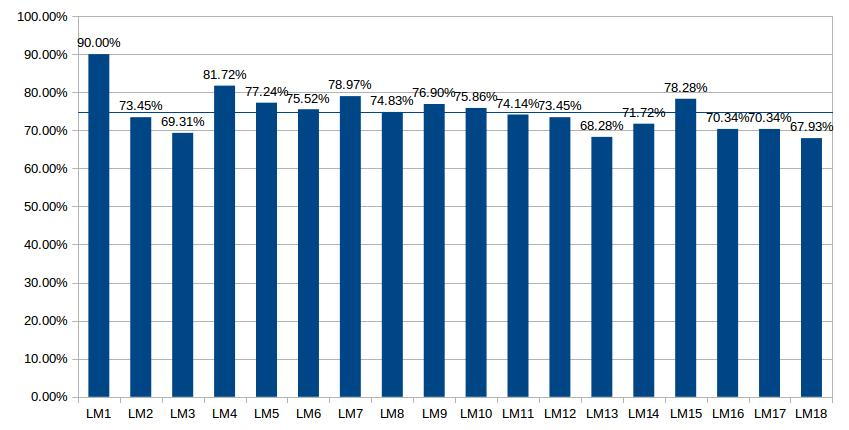
\includegraphics[scale=0.55]{images/mdSIFT}
	\caption{The proportion of well predicted landmarks on right mandibles(MAELab)}
	\label{mdfig2}
\end{figure}~\\
\subsection{Pronotum part}
The information of each training round on pronotum is shown in Table \ref{pronoloss}.
\begin{table}[h!]
	\centering
	\begin{tabular}{l p{2cm} p{2.4cm} p{2.6cm} p{2.2cm} p{2.2cm}}
	Round & Total images & Testing index (from-to) & Training index (from-to) & Training loss & Validation loss \\ \hline
	r1 & 293 & 1-33 & 34-293 & 0.00018 & 0.00019 \\ \hline
	r2 & 293 & 34-66 & remaining & 0.00019 & 0.00021 \\ \hline
	r3 & 293 & 67-99 & remaining & 0.00019 & 0.00026 \\ \hline
	r4 & 293 & 100-132 & remaining & 0.00021 & 0.00029 \\ \hline
	r5 & 293 & 133-165 & remaining & 0.00021 & 0.00029 \\ \hline
	r6 & 293 & 166-198 & remaining & 0.00019 & 0.00018 \\ \hline
	r7 & 293 & 199-231 & remaining & 0.00018 & 0.00015 \\ \hline
	r8 & 293 & 2232-264 & remaining & 0.00018 & 0.00021 \\ \hline
	r9 & 293 & 265-293 & remaining & 0.00020 & 0.00027 \\ \hline	
	\end{tabular}
	\caption{The training loss and validation loss at each training round of pronotum}
	\label{pronoloss}
\end{table}~\\[5cm]
Fig.\ref{losspronotumcurves} shows the curves of training and validation losses of two rounds on pronotum.
\begin{figure}[h!]
\centering
\subfloat[Round 1]{\label{model1loss2}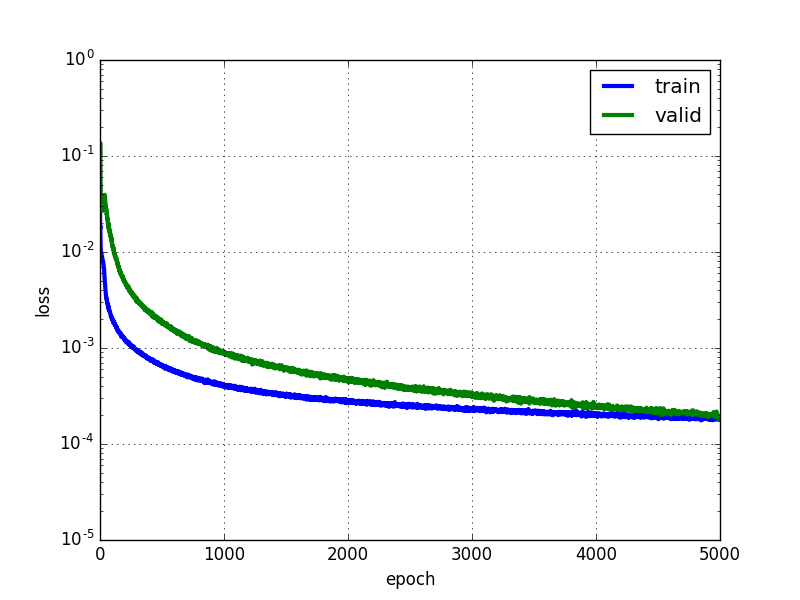
\includegraphics[width=0.5\textwidth]{./images/cnnmodel3_5000_pronotum_1000_output_v10_loss}}~~
\subfloat[Round 8]{\label{model2loss2}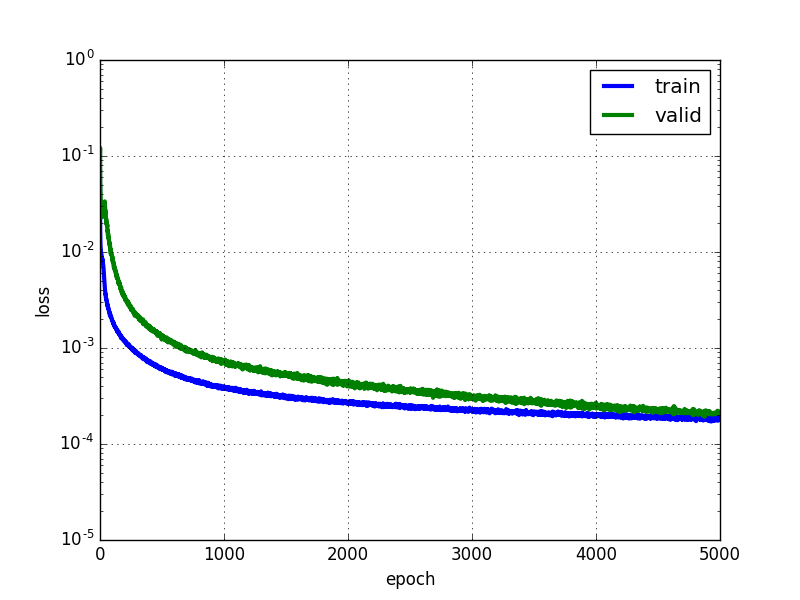
\includegraphics[width=0.5\textwidth]{./images/cnnmodel3_5000_pronotum_1000_output_v18_loss}}
\caption{The losses of two training rounds of pronotum}
\label{losspronotumcurves}
\end{figure}~\\
Table \ref{corrprono} shows the correlation coefficient between manual landmarks and predicted landmarks on pronotum part.
\begin{table}[h!]
	\centering
	\begin{tabular}{l c c}
		Method & x correlation & y correlation \\ \hline
		Pearson & $0.0.9974111$ & $0.9979428$ \\ \hline
		Spearman & $0.9944886$ & $0.9892089$ \\ \hline
		Kendall & $0.9403294$ & $0.9141635$ \\ \hline
	\end{tabular}
	\caption{The correlation between manual and predicted landmarks on pronotum images}
	\label{corrprono}
\end{table}~\\
Fig.\ref{pronofig} shows the proportions of well predicted landmarks of all pronotum images.
\begin{figure}[h!]
	\centering
	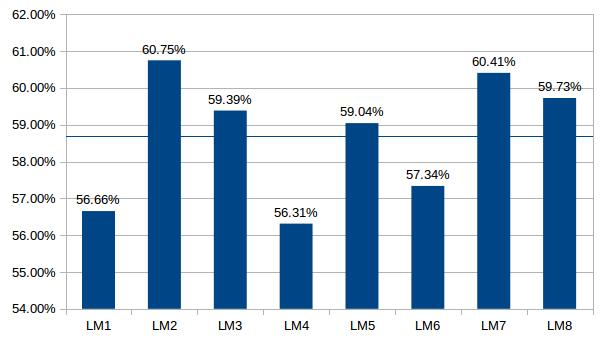
\includegraphics[scale=0.5]{images/pronotum}
	\caption{The proportion of well predicted landmarks on pronotum part}
	\label{pronofig}
\end{figure}~\\[3cm]
\subsection{Body part}
The information of each training round on body part is shown in Table \ref{bodyloss}.
\begin{table}[h!]
	\centering
	\begin{tabular}{l p{2cm} p{2.4cm} p{2.6cm} p{2.2cm} p{2.2cm}}
	Round & Total images & Testing index (from-to) & Training index (from-to) & Training loss & Validation loss \\ \hline
	r1 & 293 & 1-33 & 34-293 & 0.00019 & 0.00012 \\ \hline
	r2 & 293 & 34-66 & remaining & 0.00020 & 0.00012 \\ \hline
	r3 & 293 & 67-99 & remaining & 0.00019 & 0.00012 \\ \hline
	r4 & 293 & 100-132 & remaining & 0.00020 & 0.00011 \\ \hline
	r5 & 293 & 133-165 & remaining & 0.00018 & 0.00010 \\ \hline
	r6 & 293 & 166-198 & remaining & 0.00019 & 0.00013 \\ \hline
	r7 & 293 & 199-231 & remaining & 0.00018 & 0.00013 \\ \hline
	r8 & 293 & 2232-264 & remaining & 0.00018 & 0.00017 \\ \hline
	r9 & 293 & 265-293 & remaining & 0.00019 & 0.00012 \\ \hline	
	\end{tabular}
	\caption{The training loss and validation loss at each training round of body}
	\label{bodyloss}
\end{table}~\\
Fig.\ref{losselytrecurves} shows the curves of training and validation losses of two rounds on body part.
\begin{figure}[h!]
\centering
\subfloat[Round 1]{\label{model1loss2}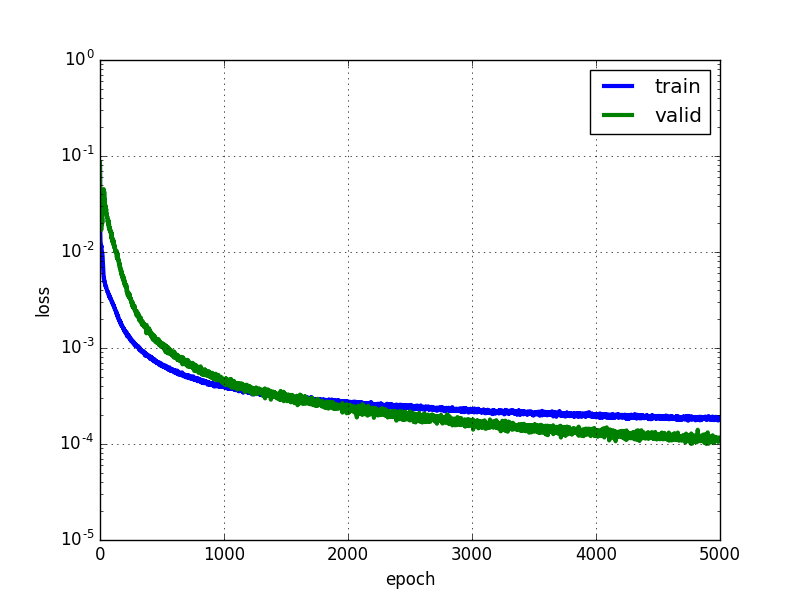
\includegraphics[width=0.5\textwidth]{./images/cnnmodel3_5000_elytre_1000_output_v10_loss}}~~
\subfloat[Round 8]{\label{model2loss2}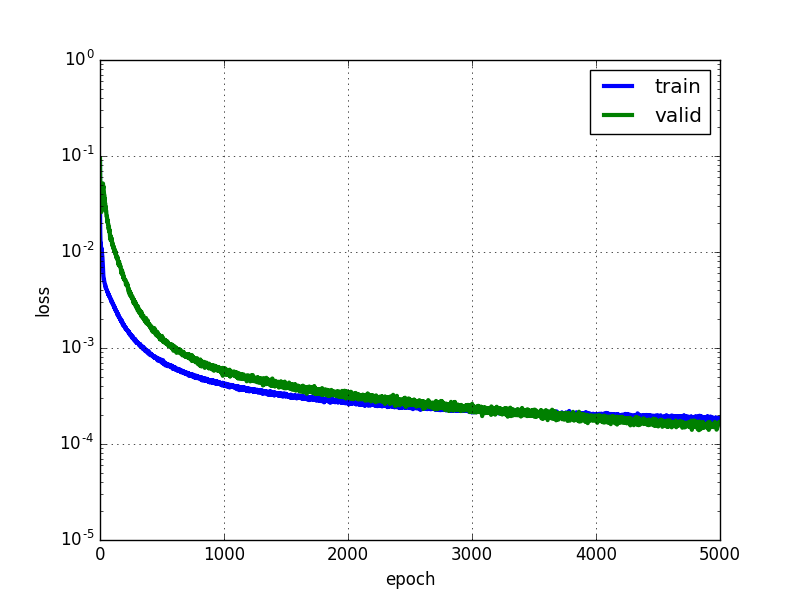
\includegraphics[width=0.5\textwidth]{./images/cnnmodel3_5000_elytre_1000_output_v18_loss}}
\caption{The losses curves of training and validation of two training rounds of body part}
\label{losselytrecurves}
\end{figure}~\\[3cm]
Table \ref{corrbody} shows the correlation coefficient between manual landmarks and predicted landmarks on body part.
\begin{table}[h!]
	\centering
	\begin{tabular}{l c c}
		Method & x correlation & y correlation \\ \hline
		Pearson & $0.9818338$ & $0.9986623$ \\ \hline
		Spearman & $0.9833374$ & $0.980597$ \\ \hline
		Kendall & $0.9032424$ & $0.8882938$ \\ \hline
	\end{tabular}
	\caption{The correlation between manual and predicted landmarks on body images}
	\label{corrbody}
\end{table}~\\
Fig.\ref{elytrefig} shows the proportions of well predicted landmarks on body part.
\begin{figure}[h!]
	\centering
	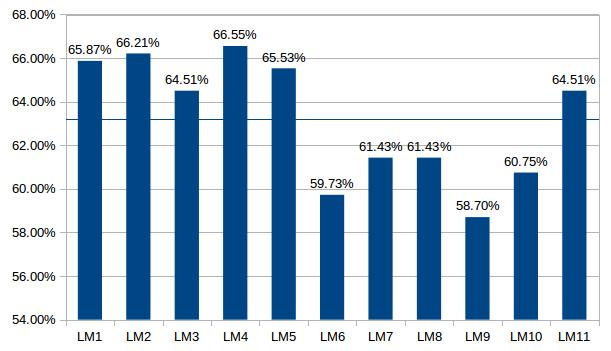
\includegraphics[scale=0.7]{images/elytre}
	\caption{The proportion of well predicted landmarks on body part}
	\label{elytrefig}
\end{figure}~\\
\subsection{Head part}
The information of each training round on head part is shown in Table \ref{headloss}.
\begin{table}[h!]
	\centering
	\begin{tabular}{l p{2cm} p{2.4cm} p{2.6cm} p{2.2cm} p{2.2cm}}
	Round & Total images & Testing index (from-to) & Training index (from-to) & Training loss & Validation loss \\ \hline
	r1 & 293 & 1-33 & 34-293 & 0.00023 & 0.00032 \\ \hline
	r2 & 293 & 34-66 & remaining & 0.00027 & 0.00044 \\ \hline
	r3 & 293 & 67-99 & remaining & 0.00026 & 0.00051 \\ \hline
	r4 & 293 & 100-132 & remaining & 0.00026 & 0.00058 \\ \hline
	r5 & 293 & 133-165 & remaining & 0.00027 & 0.00072 \\ \hline
	r6 & 293 & 166-198 & remaining & 0.00025 & 0.00050 \\ \hline
	r7 & 293 & 199-231 & remaining & 0.00023 & 0.00019 \\ \hline
	r8 & 293 & 2232-264 & remaining & 0.00024 & 0.00021 \\ \hline
	r9 & 293 & 265-293 & remaining & 0.00025 & 0.00027 \\ \hline	
	\end{tabular}
	\caption{The training loss and validation loss at each training round of head}
	\label{headloss}
\end{table}~\\
Fig.\ref{losstetecurves} shows the curves of training and validation losses of two rounds on right mandible.\\[0.1cm]
\begin{figure}[h!]
\centering
\subfloat[Round 1]{\label{model1loss2}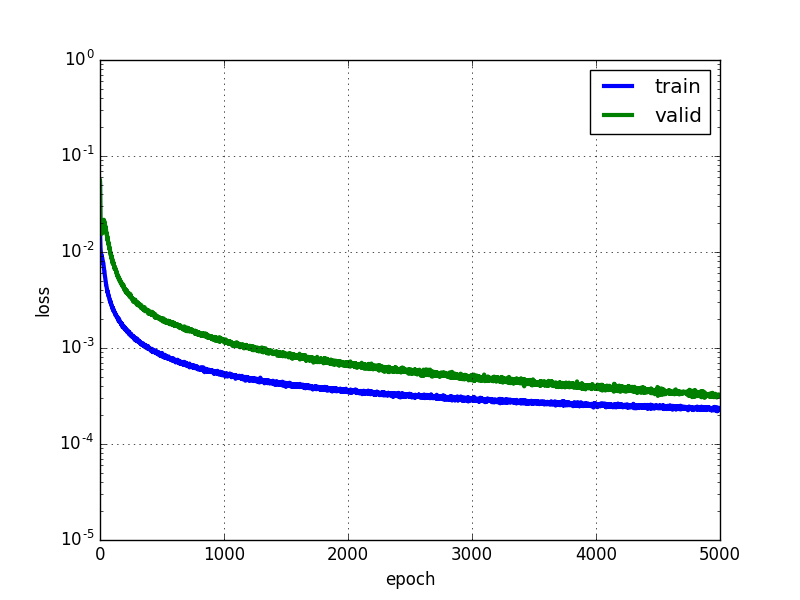
\includegraphics[width=0.5\textwidth]{./images/cnnmodel3_5000_tete_1000_output_v10_loss}}~~
\subfloat[Round 8]{\label{model2loss2}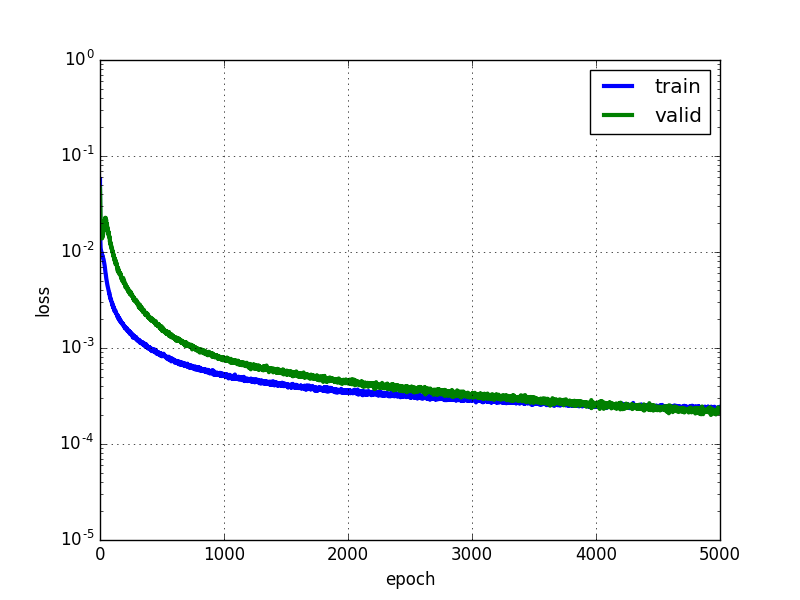
\includegraphics[width=0.5\textwidth]{./images/cnnmodel3_5000_tete_1000_output_v18_loss}}
\caption{The losses curves of training and validation of two training rounds of head part  }
\label{losstetecurves}
\end{figure}~\\
Table \ref{corrhead} shows the correlation coefficient between manual landmarks and predicted landmarks on right mandibles.
\begin{table}[h!]
	\centering
	\begin{tabular}{l c c}
		Method & x correlation & y correlation \\ \hline
		Pearson & $0.9936695$ & $0.9935629$ \\ \hline
		Spearman & $0.99080$ & $0.9944676$ \\ \hline
		Kendall & $0.9237709$ & $0.9387203$ \\ \hline
	\end{tabular}
	\caption{The correlation between manual and predicted landmarks on head images}
	\label{corrhead}
\end{table}~\\
Fig.\ref{tetefig} shows the proportions of well predicted landmarks on head part.
\begin{figure}[h!]
	\centering
	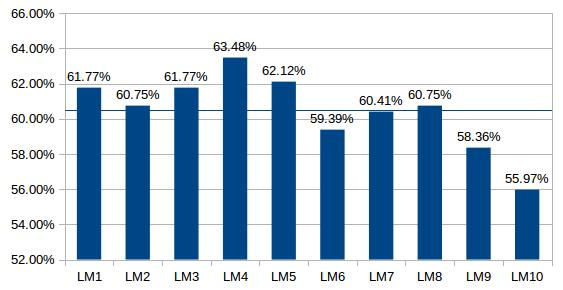
\includegraphics[scale=0.65]{images/tete}
	\caption{The proportion of well predicted landmarks on head part}
	\label{tetefig}
\end{figure}~\\

\section{Conclusions}
In this study, we proposed a CNN to predict the landmarks on beetles images. The model is evaluated on five datasets corresponding five parts of the beetle: left mandible, right mandible, pronotum, body, and head. For each dataset, the model has been trained in several times with different images data. Then, the trained model is evaluated with the corresponding test set. At the end, the coordinates of the landmarks on all the images in each dataset have been predicted. Three correlation methods have been used to calculate the coefficient between manual landmarks and predicted landmarks. Besides, a statistic based on the distance between manual and predict landmarks is also calculated. The statistic accepts the predicted landmark that has the distance (corresponding manual and itself) less than the average value (of all images). From two evaluation ways, the coefficients are enough good to precise when we consider the statistic problem. But, when we stay on the side of the image, the results are not good as we expect. Especially, when we compare this result with the result from MAELab(left and right mandible), the result from CNN model is not enough precise. We need to post-process the prediction landmarks to obtain better results.
\bibliographystyle{unsrt}
\bibliography{includes/references}
\pagebreak
\appendix
\begin{center}
\textbf{\LARGE{APPENDIX}}
\end{center}

\section{Network parameters description}
\label{apa}
The number of layers in the model are shown in Table \ref{numlayers}.
\begin{table}[h!]
	\centering
	\begin{tabular}{l p{1.2cm} p{3cm} p{2cm} p{1.2cm} p{2cm} p{2cm}}
		Model & $N^o$ layers & Input size & $N^o$ CONVs & $N^o$ POOLs & $N^o$ Dropout & $N^o$ FC \\ \hline
		model & 13 & $1 \times 256 \times 192$ & 6 & 3 & 4 & 3 \\ \hline
	\end{tabular}
	\caption{The number of layer types in each model}
	\label{numlayers}
\end{table}~\\
The detail parameters in each layer of the model are shown in Table \ref{modelparameters}.
\begin{table}[h!]
	\centering
	\begin{tabular}{l p{3cm} }
		layers &  model  \\ \hline
		input & $1 \times 256 \times 192$ \\ \hline
 		layer 1 & CONV(32,3,1,0) \\ \hline
		layer 2 & POOL(2,2,0) \\ \hline
		layer 3 & \textbf{DROP(0.1)} \\ \hline
		layer 4 & CONV(64,2,1,0) \\ \hline
		layer 5 & POOL(2,2,0) \\ \hline
		layer 6 & \textbf{DROP(0.2)} \\ \hline
		layer 7 & CONV(128,2,1,0) \\ \hline
		layer 8 & POOL(2,2,0) \\ \hline
		layer 9 & \textbf{DROP(0.3)} \\ \hline
		layer 10 & FC(1000) \\ \hline
		layer 11 & \textbf{DROP(0.5)} \\ \hline
		layer 12& FC(1000) \\ \hline
		layer 13 & FC(32/36/16/22/20) \\ \hline
	\end{tabular}
	\caption{The parameters at each layer of the model}
	\label{modelparameters}
\end{table}~\\
Which:
\begin{itemize}
	\item CONV(x,y,z,t): convolutional layer with the parameters: \textit{x = number of filters, y = size of filter matrix, z = stride value, t = padding value}
	\item POOL(y,z,t): maximum pooling layer with: \textit{y = size of filter, z = stride value, t = padding value}
	\item DROP(p): dropout layer with \textit{p is the dropout ratio}
	\item FC(x): full-connected layer with \textit{x is the number of output}
\end{itemize}
\section{Average distances}
\label{apavgdistance}
Table \ref{avgdistance} shows the average distance(between manual and predicted coordinates) of each landmark of each beetle's part. The distances are calculated in down-sample images(size of $256 \times 192$).
\begin{table}[h!]
	\centering
	\begin{tabular}{l p{3cm} p{3cm}  p{2cm}  p{2cm} p{2cm}   }
		Landmark &  Left mandible & Right mandible & Pronotum & Body & Head  \\ \hline
 		1 & 9.1267 & 9.4981 & 4.0020 & 3.8669 & 5.5280 \\ \hline
		2 & 6.7198 & 7.1657 & 4.4831 & 3.9730 & 5.1609 \\ \hline
		3 & 6.8704 & 7.2420 & 4.2959 & 3.9166 & 5.3827 \\ \hline
		4 & 6.7719 & 7.0436 & 4.3865 & 3.8673 & 5.0345 \\ \hline
		5 & 7.1250 & 7.1599 & 4.2925 & 4.0151 & 4.8393 \\ \hline
		6 & 6.9441 & 7.5699 & 5.3631 & 4.8426 & 4.4516 \\ \hline
		7 & 7.3158 & 7.4251 & 4.6360 & 5.2125 & 4.7937 \\ \hline
		8 & 7.4142 & 7.6636 & 4.936 & 5.4685 & 4.5322 \\ \hline
		9 & 7.5846 & 7.7906 & - & 5.2692 & 5.1412 \\ \hline
		10 & 7.6349 & 8.0197 & - & 4.0709 & 5.0564 \\ \hline
		11 & 7.6873 & 8.3140 & - & 3.9896 & - \\ \hline
		12 & 8.4248 & 8.1564 & - & - & - \\ \hline
		13 & 7.9983 & 8.8879 & - & - & - \\ \hline
		14 & 7.4919 & 9.1842 & - & - & - \\ \hline
		15 & 7.7903 & 8.7875 & - & - & - \\ \hline
		16 & 8.5198 & 8.3141 & - & - & - \\ \hline
		17 & - & 8.2866 & - & - & - \\ \hline
		18 & - & 8.8928 & - & - & - \\ \hline
	\end{tabular}
	\caption{The average distance of each landmark of each beetle's part}
	\label{avgdistance}
\end{table}~\\
\section{Experiment results}
\label{apb}
All of the experiment results is provided on GitHub. Each folder contains the results corresponding to each beetle's part. In each folder, we provide the losses curves, result images(first sixteen images of each test set), and the prediction landmarks(in csv file). Each folder contains:
\begin{itemize}
	%\item Folder \textbf{models} contains the output models following each training round,
	\item \textbf{Test} folder: contains the loss curves during training (and validation) and the prediction on test images (top 16) for each training round,
	\item \textbf{CSV} file: contains the information of image, index of landmark, coordinates of manual landmark$(x1,y1)$, and coordinates of predicted landmark$(x2,y2)$.
	\item The output trained model can be obtained by requesting the authors.
\end{itemize}
\end{document}